% System figure of paper v3: the hybrid of the hierarchical quaternion LSTM and LightGBM.
% Build:  cd docs/paper/manuscript_v3/figures/src && tectonic fig_system.tex && mv fig_system.pdf ..
\documentclass[tikz,border=2pt]{standalone}
\usepackage{amsmath}
\usepackage{newtxtext,newtxmath}
\usetikzlibrary{positioning,arrows.meta,fit,calc,backgrounds}
\providecommand{\bm}[1]{\boldsymbol{#1}}
\definecolor{cP}{HTML}{0072B2}\definecolor{cM}{HTML}{E69F00}\definecolor{cC}{HTML}{009E73}\definecolor{cG}{HTML}{D55E00}
\definecolor{wa}{HTML}{0072B2}\definecolor{wb}{HTML}{E69F00}\definecolor{wc}{HTML}{009E73}\definecolor{wd}{HTML}{CC79A7}
\begin{document}
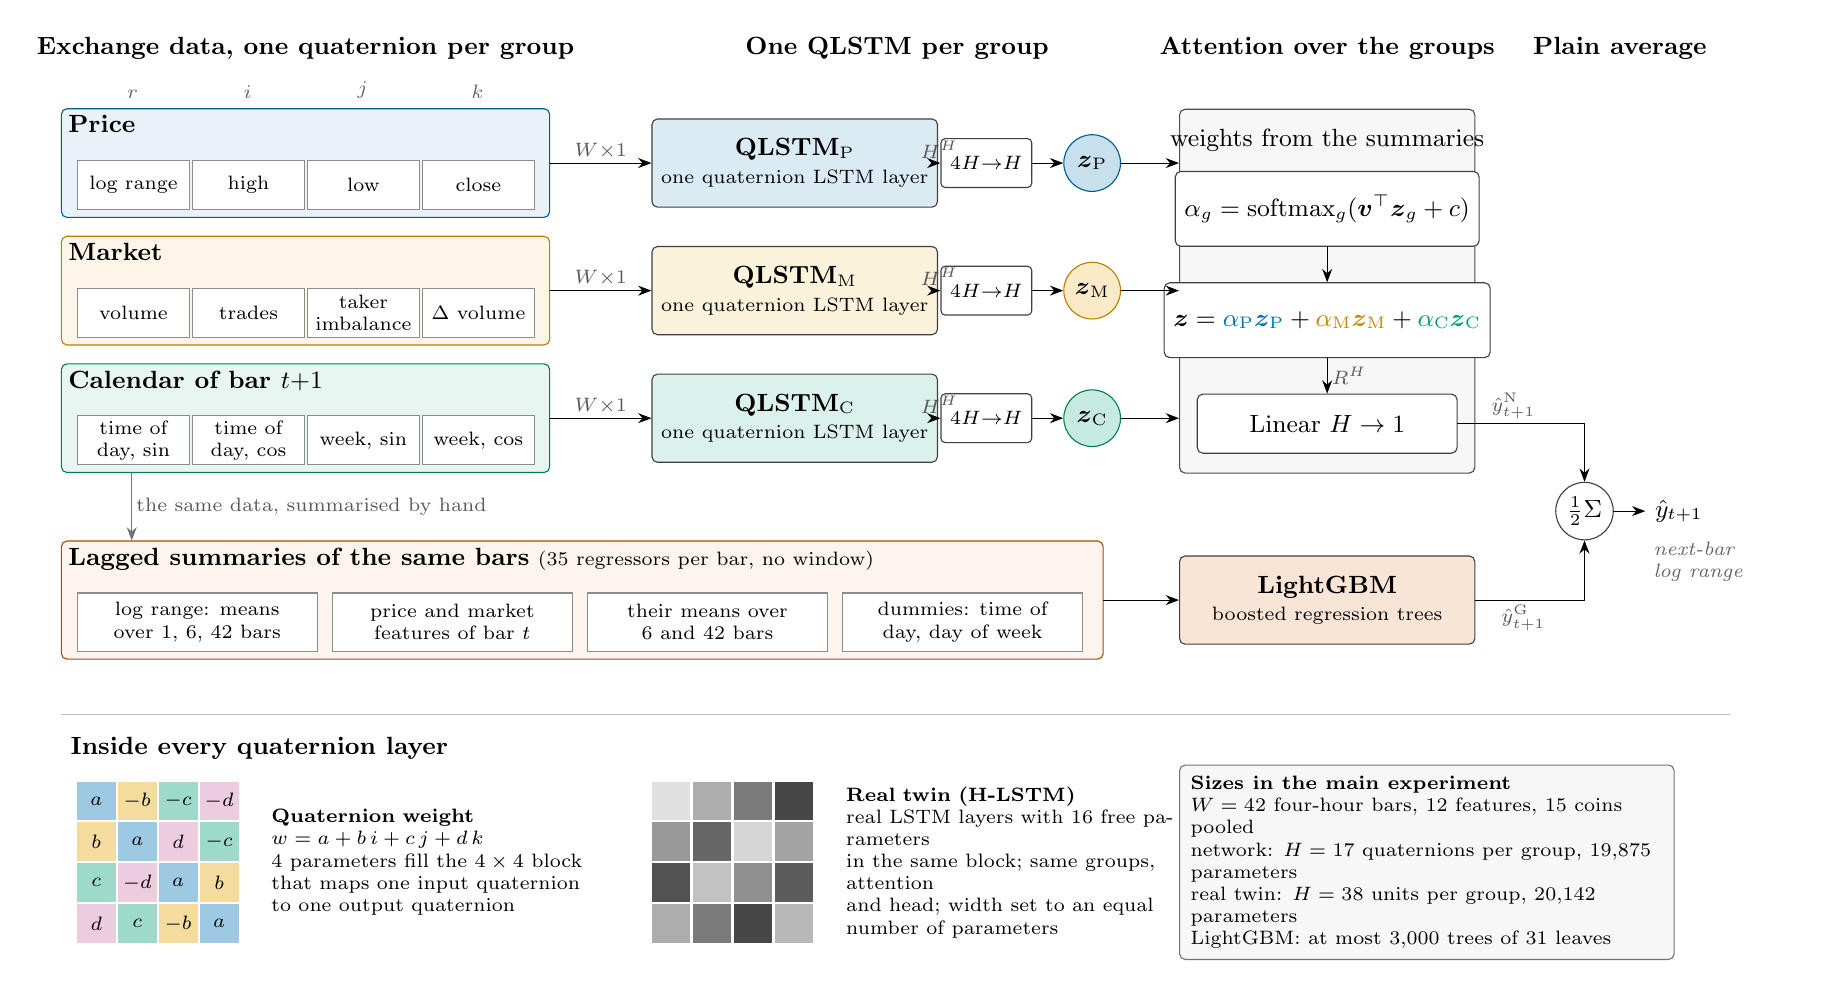
\begin{tikzpicture}[
  font=\small, >=Stealth, line cap=round,
  stage/.style={font=\bfseries\small, anchor=south},
  cell/.style={draw=black!45, fill=white, minimum width=1.42cm, minimum height=0.62cm, inner sep=1pt,
               font=\scriptsize, align=center, text width=1.36cm},
  comp/.style={font=\scriptsize\itshape, text=black!60},
  note/.style={font=\scriptsize\itshape, text=black!60, align=flush left, anchor=north west},
  blk/.style={draw=black!70, rounded corners=2pt, fill=black!4, align=center, inner sep=3pt},
  shp/.style={font=\scriptsize, text=black!65, inner sep=1.5pt},
  wcell/.style={draw=white, line width=0.8pt, minimum size=0.52cm, inner sep=0pt, font=\scriptsize}]

% ---------------------------------------------------------------- inputs: one quaternion per group and bar
\foreach \g/\name/\col/\y/\a/\b/\c/\d in {
  P/{Price}/cP/0/{log range}/{high}/{low}/{close},
  M/{Market}/cM/-1.62/{volume}/{trades}/{taker imbalance}/{$\Delta$ volume},
  C/{Calendar of bar $t{+}1$}/cC/-3.24/{time of day, sin}/{time of day, cos}/{week, sin}/{week, cos}} {
  \node[draw=\col!80!black, rounded corners=2pt, fill=\col!9, minimum width=6.20cm, minimum height=1.38cm,
        anchor=west] (g\g) at (0,\y) {};
  \node[anchor=north west, font=\small, inner sep=2.5pt] at (g\g.north west) {\textbf{\name}};
  \foreach \k/\txt in {0/\a,1/\b,2/\c,3/\d}
    \node[cell, anchor=south west] at ($(g\g.south west)+(0.20+\k*1.46,0.10)$) {\txt};
}
\foreach \k/\lab in {0/r,1/i,2/j,3/k}
  \node[comp, anchor=south] at ($(gP.north west)+(0.91+\k*1.46,0.0)$) {$\lab$};
\node[stage] at ($(gP.north)+(0,0.50)$) {Exchange data, one quaternion per group};

% ---------------------------------------------------------------- network: group encoders
\foreach \g/\col/\y in {P/cP/0, M/cM/-1.62, C/cC/-3.24} {
  \node[draw=black!75, rounded corners=2pt, fill=\col!14, minimum width=2.95cm, minimum height=1.12cm,
        anchor=west, align=center] (e\g) at (7.50,\y) {\textbf{QLSTM$_{\mathrm{\g}}$}\\[-1pt]{\scriptsize one quaternion LSTM layer}};
  \node[draw=black!75, rounded corners=1.5pt, fill=white, minimum width=0.95cm, minimum height=0.62cm,
        anchor=west, font=\scriptsize] (p\g) at (11.17,\y) {$4H{\to}H$};
  \node[draw=\col!80!black, circle, fill=\col!22, minimum size=0.72cm, inner sep=0pt, anchor=west]
        (z\g) at (12.73,\y) {$\bm{z}_{\mathrm{\g}}$};
  \draw[->] (g\g.east) -- node[shp, above] {$W{\times}1$} (e\g.west);
  \draw[->] (e\g.east) -- node[shp, above] {$\mathbb{H}^{H}$} (p\g.west);
  \draw[->] (p\g.east) -- (z\g.west);
}
\node[stage] at ($(eP.north |- gP.north)+(1.3,0.50)$) {One QLSTM per group};

% ---------------------------------------------------------------- network: attention over the groups
\node[blk, minimum width=3.75cm, minimum height=4.62cm, anchor=north west, fill=black!3]
  (fus) at (14.20,0.69) {};
\node[anchor=north, font=\small, align=center] (ft) at ($(fus.north)+(0,-0.14)$)
  {weights from the summaries};
\node[draw=black!75, rounded corners=2pt, fill=white, minimum width=3.3cm, minimum height=0.95cm,
      align=center, anchor=north] (fa) at ($(ft.south)+(0,-0.12)$)
  {$\alpha_g=\operatorname{softmax}_g(\bm{v}^{\top}\bm{z}_g+c)$};
\node[draw=black!75, rounded corners=2pt, fill=white, minimum width=3.3cm, minimum height=0.95cm,
      align=center, anchor=north] (fs) at ($(fa.south)+(0,-0.45)$)
  {$\bm{z}=\textcolor{cP}{\alpha_{\mathrm{P}}\bm{z}_{\mathrm{P}}}+\textcolor{cM!85!black}{\alpha_{\mathrm{M}}\bm{z}_{\mathrm{M}}}
     +\textcolor{cC}{\alpha_{\mathrm{C}}\bm{z}_{\mathrm{C}}}$};
\node[draw=black!75, rounded corners=2pt, fill=white, minimum width=3.3cm, minimum height=0.75cm,
      align=center, anchor=north] (fl) at ($(fs.south)+(0,-0.45)$) {Linear $H\to 1$};
\draw[->] (fa.south) -- (fs.north);
\draw[->] (fs.south) -- node[shp, right] {$\mathbb{R}^{H}$} (fl.north);
\foreach \g in {P,M,C} \draw[->] (z\g.east) -- (z\g.east -| fus.west);
\node[stage] at ($(fus.north |- gP.north)+(0,0.50)$) {Attention over the groups};

% ---------------------------------------------------------------- LightGBM branch
\node[draw=cG!80!black, rounded corners=2pt, fill=cG!7, minimum width=13.23cm, minimum height=1.50cm,
      anchor=west] (lag) at (0,-5.55) {};
\node[anchor=north west, font=\small, inner sep=2.5pt] at (lag.north west)
  {\textbf{Lagged summaries of the same bars} {\scriptsize(35 regressors per bar, no window)}};
\foreach \k/\txt in {0/{log range: means\\over 1, 6, 42 bars}, 1/{price and market\\features of bar $t$},
                     2/{their means over\\6 and 42 bars}, 3/{dummies: time of\\day, day of week}}
  \node[draw=black!45, fill=white, minimum width=3.05cm, minimum height=0.74cm, inner sep=1pt, font=\scriptsize,
        align=center, anchor=south west] at ($(lag.south west)+(0.20+\k*3.24,0.10)$) {\txt};
\node[draw=black!75, rounded corners=2pt, fill=cG!16, minimum width=3.75cm, minimum height=1.12cm,
      anchor=west, align=center] (gbm) at (14.20,-5.55) {\textbf{LightGBM}\\[-1pt]{\scriptsize boosted regression trees}};
\draw[->] (lag.east) -- (gbm.west);
\draw[->, black!55] ($(gC.south west)+(0.9,0)$) -- node[shp, right, pos=0.5] {the same data, summarised by hand} ($(lag.north west)+(0.9,0)$);

% ---------------------------------------------------------------- average
\node[draw=black!75, circle, fill=white, inner sep=1.5pt, font=\small] (avg) at (19.35,-4.42) {$\tfrac12\Sigma$};
\node[anchor=west, align=left] (yh) at ($(avg.east)+(0.40,0)$) {$\hat y_{t+1}$};
\node[note, text width=2.0cm, anchor=north west] at ($(yh.south west)+(-0.02,0.0)$) {next-bar\\log range};
\draw[->] (fl.east) -| node[shp, above, pos=0.22] {$\hat y^{\mathrm{N}}_{t+1}$} (avg.north);
\draw[->] (gbm.east) -| node[shp, below, pos=0.22] {$\hat y^{\mathrm{G}}_{t+1}$} (avg.south);
\draw[->] (avg.east) -- (yh.west);
\node[stage] at ($(avg.north |- gP.north)+(0.45,0.50)$) {Plain average};

% ---------------------------------------------------------------- inset: what a quaternion layer shares
\begin{scope}[shift={(0.0,-8.05)}]
  \node[anchor=west, font=\bfseries\small] at (0,0.62) {Inside every quaternion layer};
  \foreach \r/\row in {0/{wa/a,wb/{-b},wc/{-c},wd/{-d}}, 1/{wb/b,wa/a,wd/d,wc/{-c}},
                       2/{wc/c,wd/{-d},wa/a,wb/b}, 3/{wd/d,wc/c,wb/{-b},wa/a}} {
    \foreach \col/\txt [count=\ci from 0] in \row
      \node[wcell, fill=\col!38] at (0.45+\ci*0.52,-0.05-\r*0.52) {$\txt$};
  }
  \node[anchor=west, align=left, text width=4.3cm, font=\scriptsize] at (2.55,-0.83)
    {\textbf{Quaternion weight}\\$w=a+b\,i+c\,j+d\,k$\\4 parameters fill the $4\times4$ block\\that maps one input quaternion\\to one output quaternion};
  \foreach \r in {0,1,2,3} \foreach \ci in {0,1,2,3} {
    \pgfmathtruncatemacro{\shade}{12+mod(\r*7+\ci*5,16)*4}
    \node[wcell, fill=black!\shade] at (7.75+\ci*0.52,-0.05-\r*0.52) {};
  }
  \node[anchor=west, align=left, text width=4.3cm, font=\scriptsize] at (9.85,-0.83)
    {\textbf{Real twin (H-LSTM)}\\real LSTM layers with 16 free parameters\\in the same block; same groups, attention\\and head; width set to an equal\\number of parameters};
  \node[draw=black!55, rounded corners=2pt, fill=black!3, anchor=west, align=flush left, text width=6.0cm,
        font=\scriptsize, inner sep=4pt] at (14.20,-0.83)
    {\textbf{Sizes in the main experiment}\\$W=42$ four-hour bars, 12 features, 15 coins pooled\\network: $H=17$ quaternions per group, 19{,}875 parameters\\real twin: $H=38$ units per group, 20{,}142 parameters\\LightGBM: at most 3{,}000 trees of 31 leaves};
\end{scope}
\begin{scope}[on background layer]
  \draw[black!25, line width=0.4pt] (0,-7.00) -- (21.2,-7.00);
\end{scope}
\end{tikzpicture}
\end{document}
